\documentclass{rosenpass-beamer}

\usepackage[ngerman]{babel}
\usepackage[autostyle]{csquotes}
\usepackage{emoji}
%\usepackage{dirtytalk}
\let\say\enquote

\usepackage{xurl}

\urlstyle{same}

\usepackage{textcomp}

\usetikzlibrary{positioning,decorations.pathreplacing,svg.path}

\definecolor{RPPink}{rgb}{274,4,132}
\definecolor{RPOrange}{rgb}{255, 166, 48}
\definecolor{RPAquamarine}{rgb}{255, 166, 48}
\definecolor{RPLightGray}{rgb}{160, 159, 164}
\definecolor{RPTurquoise}{rgb}{114, 161, 229}

\usepackage{bbding}
\newcommand*\itemtick{\item[\Checkmark]}
\newcommand*\itemfail{\item[\XSolidBrush]}

\newcommand*{\heading}[1]{
  {
    \hspace*{-0.5cm}#1
    \vspace{1.0em}
  }
}

\title{Rosenpass}
%\subtitle{VPN \& Struktur für Translationsforschung in der Kryptografie}
\author{
Wanja Zaeske, Stephan Ajuvo, Marei Peischl, Benjamin Lipp, Lisa~Schmidt, Karolin Varner
}
\institute{\url{https://rosenpass.eu}}


\conference{Formosa Retreat Juli 2023}
\date{2023-07-11}

\parskip\smallskipamount

\ExplSyntaxOn
\newcommand*{\sourcename}{Quelle}
\newcommand*{\sourcesep}{:~}

\newcommand*{\imgNote}[1]{\begin{center}\setlength{\parskip}{0pt}\tiny\raggedright#1\end{center}}
\NewDocumentCommand{\mgSource}{smm}{%
%\hbox_set:Nn \l_tmpa_box {#1}

\hbox_set:Nn \l_tmpa_box {#2}

\hbox_set:Nn \l_tmpa_box {
\dim_set:Nn \l_tmpa_dim {\box_ht:N \l_tmpa_box}
\hbox_unpack_drop:N \l_tmpa_box \rotatebox{90}{\parbox{\dim_eval:n {\IfBooleanTF {#1} {\linewidth} {\l_tmpa_dim}}}{\tiny\raggedright\sourcename\sourcesep#3}}
}
\box_use:N \l_tmpa_box
}
\ExplSyntaxOff

% reduce itemize indent
\setlength{\leftmargini}{0pt}

\usepackage{biblatex}
\addbibresource{sources.bib}


%namepartpicturesetup
\ExplSyntaxOn
\int_new:N \l__ptxcd_namepart_int
\fp_new:N \l__ptxcd_namepos_fp
\def\namepartsep{1.1}
\dim_new:N \l__ptxcd_namepart_sep_dim
\dim_set:Nn \l__ptxcd_namepart_sep_dim  {3mm}

\newcommand*{\namepart}[2][0]{
	\int_set:Nn \l__ptxcd_namepart_int {\clist_count:n {#2}}
	\begin{scope}[xshift=#1]
	\fp_set:Nn \l__ptxcd_namepos_fp {\l__ptxcd_namepart_int / 2}
	\keyval_parse:nnn {\__ptxcd_namepart_item:nn {}}{ \__ptxcd_namepart_item:nn } {#2}
	\end{scope}
}

\newcommand*{\SingleNamePart}[4][0]{
		\node[rounded~corners,fill=rosenpass-lightblue] (#2) at (#1,-.7) {\ttfamily#3};
		\node[above] at (#2.north) {\footnotesize #4};
}

\cs_new:Nn \__ptxcd_namepart_item:nn {
	\fp_sub:Nn \l__ptxcd_namepos_fp {1}
	\node[rounded~corners,fill=rosenpass-lightblue] (#1) at (0,\fp_use:N \l__ptxcd_namepos_fp * \namepartsep) {\ttfamily#1};
	\node[above] at (#1.north) {\footnotesize #2};
}


\newcommand*{\namebraceleft}[2] {
	\draw[decorate]([xshift=-\l__ptxcd_namepart_sep_dim]#2.south~west)--([xshift=-\l__ptxcd_namepart_sep_dim]#1.north~west) ;
}

\newcommand*{\namebraceright}[2]{
	\draw[decorate]([xshift=\l__ptxcd_namepart_sep_dim]#1.north~east) --([xshift=\l__ptxcd_namepart_sep_dim]#2.south~east);
}
\ExplSyntaxOff

\graphicspath{{}{graphics/}}

\begin{document}

\maketitle

\begin{frame}{Hello, I am Karolin Varner}
\begin{itemize}
  \item Worked with about every industry tech; incl. Java Web Apps, Microcontrollers, and legacy database system from the 80s
  \item Did a lot of project management and some people management
  \item Did a lot of open-source development, privacy- and internet politics activism
  \item Planning to get involved in the Formosa space
\end{itemize}
\end{frame}

\begin{frame}{Rosenpass}

\vspace{0.5em}
\begin{columns}[t]
\begin{column}{.30\textwidth}
\heading{WireGuard}
\begin{itemize}
  \itemtick Session-key secrecy
  \itemtick \dots
  \itemtick Identity Hiding
  \itemfail \textbf{Non-Interruptability} \footnote[frame]{Assuming a trusted system time}
  \itemfail \textbf{Post-Quantum Security}
\end{itemize}
\end{column}

\begin{column}{.30\textwidth}
\heading{
  PQ WireGuard
  \footnote[frame]{
	  Hülsing, Ning, Schwabe, Weber, Zimmermann. “Post-quantum WireGuard”. https://ia.cr/2020/379
	}
}
\begin{itemize}
  \itemtick \textbf{Post-Quantum Security}
  \itemfail \textbf{Hybrid security}
  \itemfail \textbf{Non-Interruptability} \footnote[frame]{Assuming a PSK}
\end{itemize}
\end{column}

\begin{column}{.30\textwidth}
\heading{Rosenpass}
\begin{itemize}
  \itemtick \textbf{Non-Interruptability} \footnote[frame]{Through cookies}
  \itemtick \textbf{Hybrid security} \footnote[frame]{Used together with standard WireGuard}
\end{itemize}
\end{column}

\end{columns}
\vspace{1.5em}

\end{frame}

%\begin{frame}{Rosenpass/WireGuard integration}
  \begingroup
\shorthandoff{"}
\shorthandoff*{"}


\definecolor{wireguard}{HTML}{88171a}

\def\keysvg{svg "m58.981 1976.4c-114.55-14.22-201.79-85.99-201.79-172.27 0-96.48 109.11-174.82 243.5-174.82 134.39 0 243.5 78.34 243.5 174.82 0 83.56-81.82 153.5-191.04 170.75v236.82c0 1.36-0.05 2.7-0.17 4.03 0.12 1.21 0.17 2.44 0.17 3.68 0 21.73-17.64 39.38-39.38 39.38h-129.66c-21.74 0-39.38-17.65-39.38-39.38s17.64-39.38 39.38-39.38h74.87v-43.27h-32.49c-21.73 0-39.38-17.65-39.38-39.38s17.65-39.38 39.38-39.38h32.49zm41.71-259.68c-75 0-135.88 39.17-135.88 87.41 0 48.25 60.88 87.41 135.88 87.41 74.99 0 135.88-39.16 135.88-87.41 0-48.24-60.89-87.41-135.88-87.41z"}
\def\brokenkeysvg{ svg "m 1830.23,1724.48 c 0.76,-0.05 1.52,-0.07 2.29,-0.07 h 32.49 v -81.6 c -114.55,-14.22 -201.79,-85.99 -201.79,-172.27 0,-96.48 109.11,-174.82 243.5,-174.82 134.39,0 243.5,78.34 243.5,174.82 0,83.56 -81.83,153.5 -191.04,170.75 v 236.82 c 0,1.36 -0.05,2.7 -0.17,4.03 0.12,1.21 0.17,2.44 0.17,3.68 0,21.73 -17.64,39.38 -39.37,39.38 h -70.91 l 9.5,-35.84 -30.45,-8.07 12.66,-17.87 -23.96,-16.98 h 48.36 v -27.25 l 16.81,6.08 14.01,-38.7 -85.36,-30.91 23.23,-2.84 z m 76.49,-341.35 c -74.99,0 -135.88,39.17 -135.88,87.41 0,48.25 60.89,87.41 135.88,87.41 74.99,0 135.88,-39.16 135.88,-87.41 0,-48.24 -60.89,-87.41 -135.88,-87.41 z"}

\def\lightningsvg{svg "m 118.00601,351.54023 79.56815,-0.29104 -51.98004,64.5795 29.85293,16.32215 -72.54346,92.49833 26.51919,-68.43977 -35.030831,-16.27188 z";}
\ExplSyntaxOn
\box_new:N  \l_lightning_box
\hbox_set:Nn \l_lightning_box {\tikz[rotate=180,scale=.15,sharp~corners]{\fill[wireguard,use~as~bounding~box]\lightningsvg}}

\newcommand*{\LightningIconWireGuard}{\box_use:N \l_lightning_box}

\box_new:N  \l_lightning_rosenpass_box
\hbox_set:Nn \l_lightning_rosenpass_box {\tikz[rotate=180,scale=.15,sharp~corners]{\fill[rosenpass-blue,use~as~bounding~box]\lightningsvg}}
\newcommand*{\LightningIconRosenpass}{\box_use:N \l_lightning_rosenpass_box}

\box_new:N \l_key_rosenpass_box
\box_new:N \l_broken_key_rosenpass_box

\hbox_set:Nn  \l_key_rosenpass_box  {
\includegraphics[width=3mm]{key-opt}}

\hbox_set:Nn  \l_broken_key_rosenpass_box  {
\includegraphics[width=3mm]{broken-key}}%{\tikz[rotate=180,scale=.02,sharp~corners]{\fill[rosenpass-blue,use~as~bounding~box]\brokenkeysvg}}


\newcommand*{\KeyIcon}{\box_use:N   \l_key_rosenpass_box }

\newcommand*{\BrokenKeyIcon}{\box_use:N  \l_broken_key_rosenpass_box }

\colorlet{rosenpass}{rosenpass-blue}

\setbeamertemplate{frametitle}{
\nointerlineskip
	\vspace*{-\dp\strutbox}
	\usebeamercolor{frametitle}
	\makebox[\linewidth][r]{\rlap{\raisebox{-.95\height}[0pt][0pt]{\box_use:N \g__ptxcd_logo_box}}\hspace{-.5em}}\par\nointerlineskip
 \vspace{\dp\strutbox}
}

\ExplSyntaxOff


\begin{frame}{\strut}
\vspace{3mm}
  \begin{tikzpicture}[rosenpass-diagram,
  handshake/.style={every node/.append style={boxed,sharp corners},<->}]
  \begin{scope}
  \node[inner sep=2mm,fill=rosenpass-blue,text=white,above=2\baselineskip,minimum width=5.5cm]at (0,0) {\LARGE Rosenpass};
  	\draw[initiator] (-2,0) node(alice){Alice}  ++(0,.1)to
  	 coordinate[pos=.1](hs1-y)
  	  	coordinate[pos=.3](hs3-y)
  	coordinate[pos=.3](disci-y)
  	coordinate[pos=.8](hs2-y)
%  	coordinate[pos=.9](ack-y)
  	+(0,-.4\textheight)
	  	   	+(0,-.6\textheight)
	  	   	--
	  	   	+(0,-.8\textheight);
  	\draw[responder] (2,0) node(bob){Bob} ++(0,.1)to+(0,-.4\textheight)
  	  	   	+(0,-.6\textheight)
  	  	   	--
  	  	   	+(0,-.8\textheight);;
  	\foreach \y in {-.5,-1.5,-2.5,-5} {\draw[rosenpass-blue,handshake]
  		(0,\y-|alice) --node(handshake\y){Handshake} (0,\y-|bob); 
  	}
  	
  	\node at (0,-2.55) {\LightningIconRosenpass};
  	\draw[rosenpass-blue,loosely dotted] (0,-3)--(0,-4.5);
  	\end{scope}

  	   \begin{scope}[xshift=6cm]
  	     \node[inner sep=2mm,fill=wireguard,text=white,above=2\baselineskip,minimum width=5.5cm]at (0,0) {\LARGE WireGuard};
  	   	\draw[initiator] (-2,0) node(alice2){Alice}  ++(0,.1)to
  	   	 coordinate[pos=.1](hs1-y)
  	   	  	coordinate[pos=.3](hs3-y)
  	   	coordinate[pos=.3](disci-y)
  	   	coordinate[pos=.8](hs2-y)
  	 %  	coordinate[pos=.9](ack-y)
  	   	+(0,-.45\textheight)
  	   	+(0,-.65\textheight)
  	   	--
  	   	+(0,-.8\textheight);
  	   	\draw[responder] (2,0) node(bob2){Bob} ++(0,.1)to+(0,-.45\textheight)  	   	+(0,-.65\textheight)
  	   	  	   	--
  	   	  	   	+(0,-.8\textheight);
  	   	\foreach \y in {-1,-2,-5.5} {\draw[wireguard,handshake]
  	   		(0,\y-|alice2) --node{Handshake} (0,\y-|bob2); 
  	   	}
  	   	  	 %  	
  	   	  	   	\foreach \y in {-3,-4} {\draw[wireguard,handshake,rosenpass dashed]
  	   	  	   		(0,\y-|alice2) --node[solid]{Handshake} (0,\y-|bob2); 
  	   	  	   	}

  	   	\node[wireguard] at (-.1,-3.05) {\LightningIconWireGuard};
  	   	\node[wireguard] at (-.1,-4.05) {\LightningIconWireGuard};
  	   	\draw[wireguard,loosely dotted] (0,-4.5)--(0,-5);
  	   	\end{scope}
  	   	 
  	   	 \begin{scope}[rosenpass-blue,every node/.append style={fill=white,text width=3mm,font=\tiny}]
  	   	 \draw(0,-.5-|bob)--node{PSK \KeyIcon}(0,-1-|alice2);
  	 	 \draw(0,-1.5-|bob)--node{PSK \KeyIcon}(0,-2-|alice2);
  	 	  \draw(0,-5-|bob)--node{PSK \KeyIcon}(0,-5.5-|alice2);
	 	 \draw(0,-2.5-|bob)--node{\centering!\\\BrokenKeyIcon\makebox[0pt][c]{! Kaputter Schlüssel}}(0,-3-|alice2);
		\end{scope}
  \end{tikzpicture}
\end{frame}
\endgroup
%\end{frame}

\begin{frame}{Rosenpass can be used right now}
  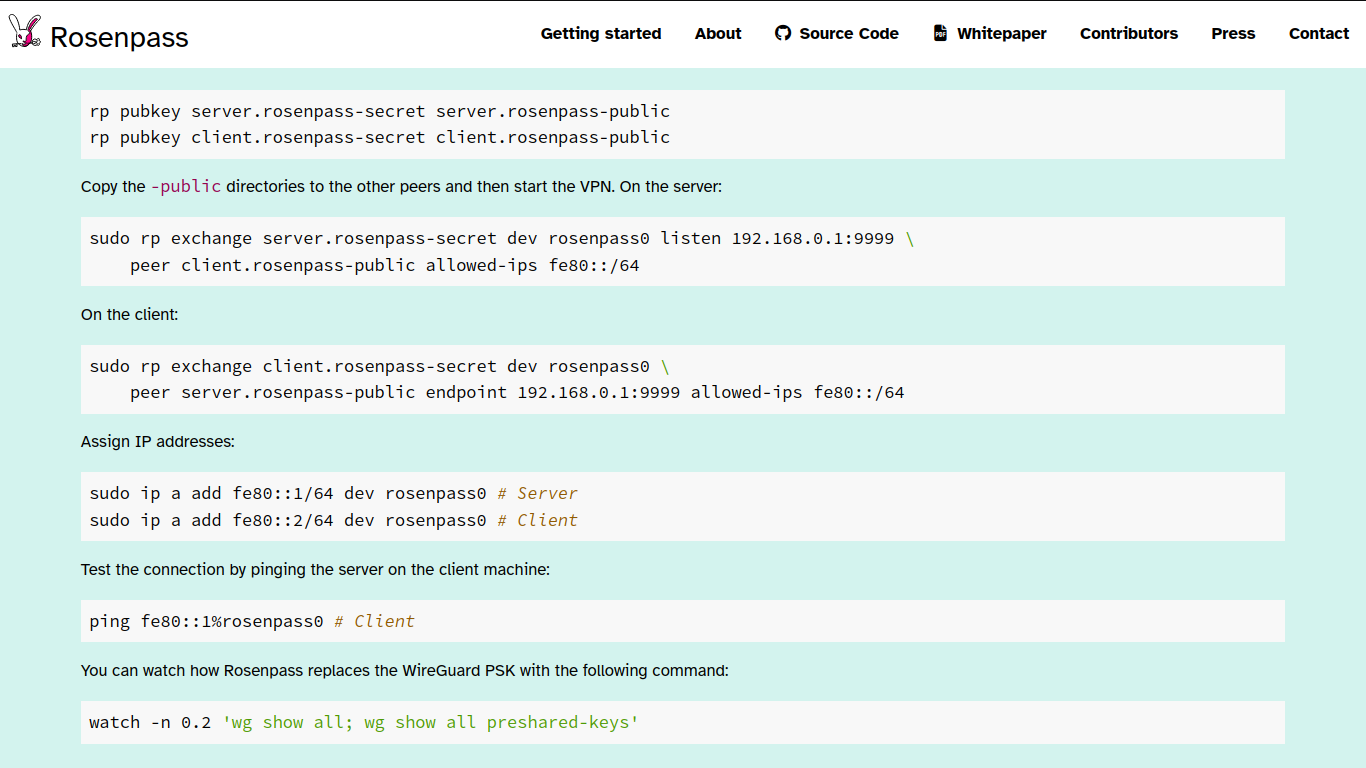
\includegraphics[height=.9\textheight]{assets/2023-03-20-rg-tutorial-screenshot.png}
\end{frame}

\begin{frame}{ProVerif in Technicolor}
  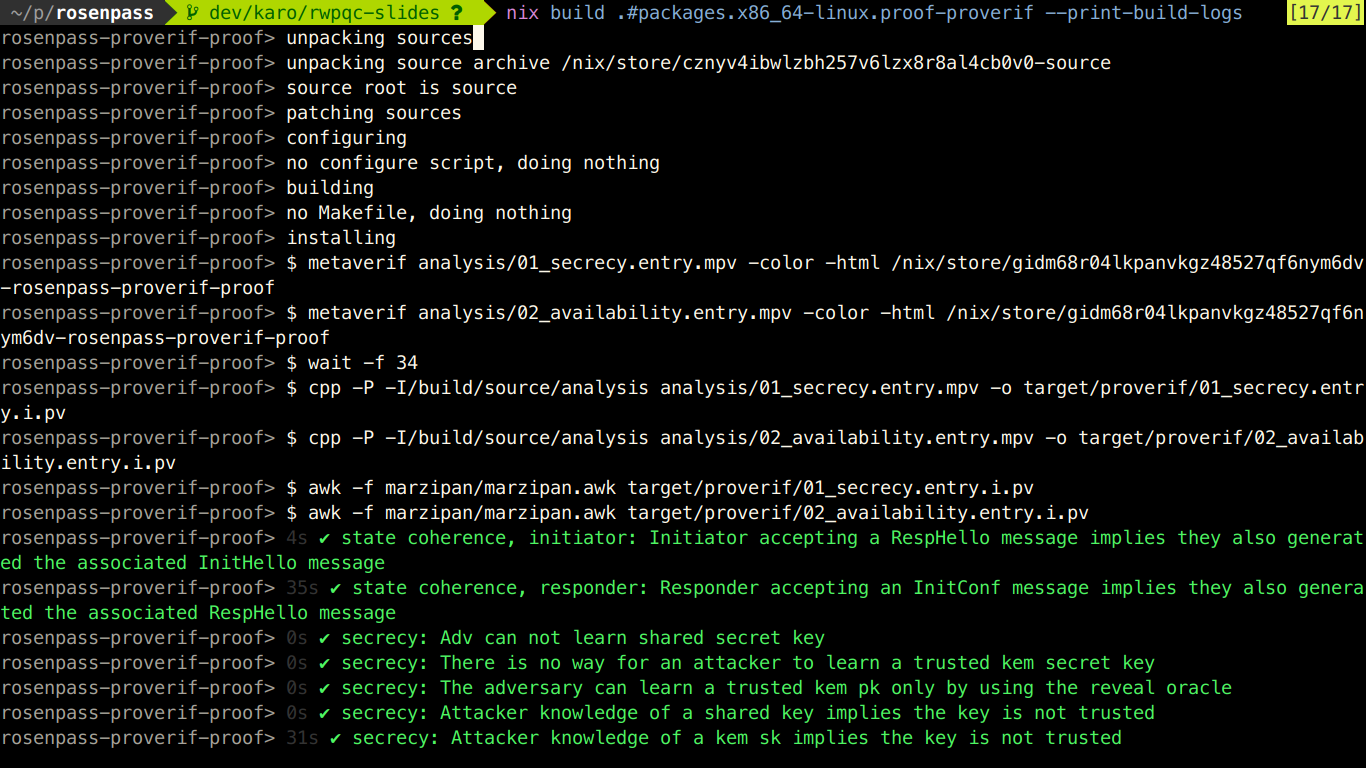
\includegraphics[height=.9\textheight]{assets/2023-03-20-symbolic-analysis-screenshot.png}
\end{frame}

\begin{frame}{Having worked in industry has some advantages}
\begin{itemize}
  \item Knowing how to get projects done
  \item Coordinating teams instead of working on my own
  \item Product and user focused perspective
  \item Building tools that I can use to be more productive
  \item Open-Source approach: How to catch new contributors
\end{itemize}
\end{frame}

\begin{frame}{The spec makes it easy to implement Rosenpass}
  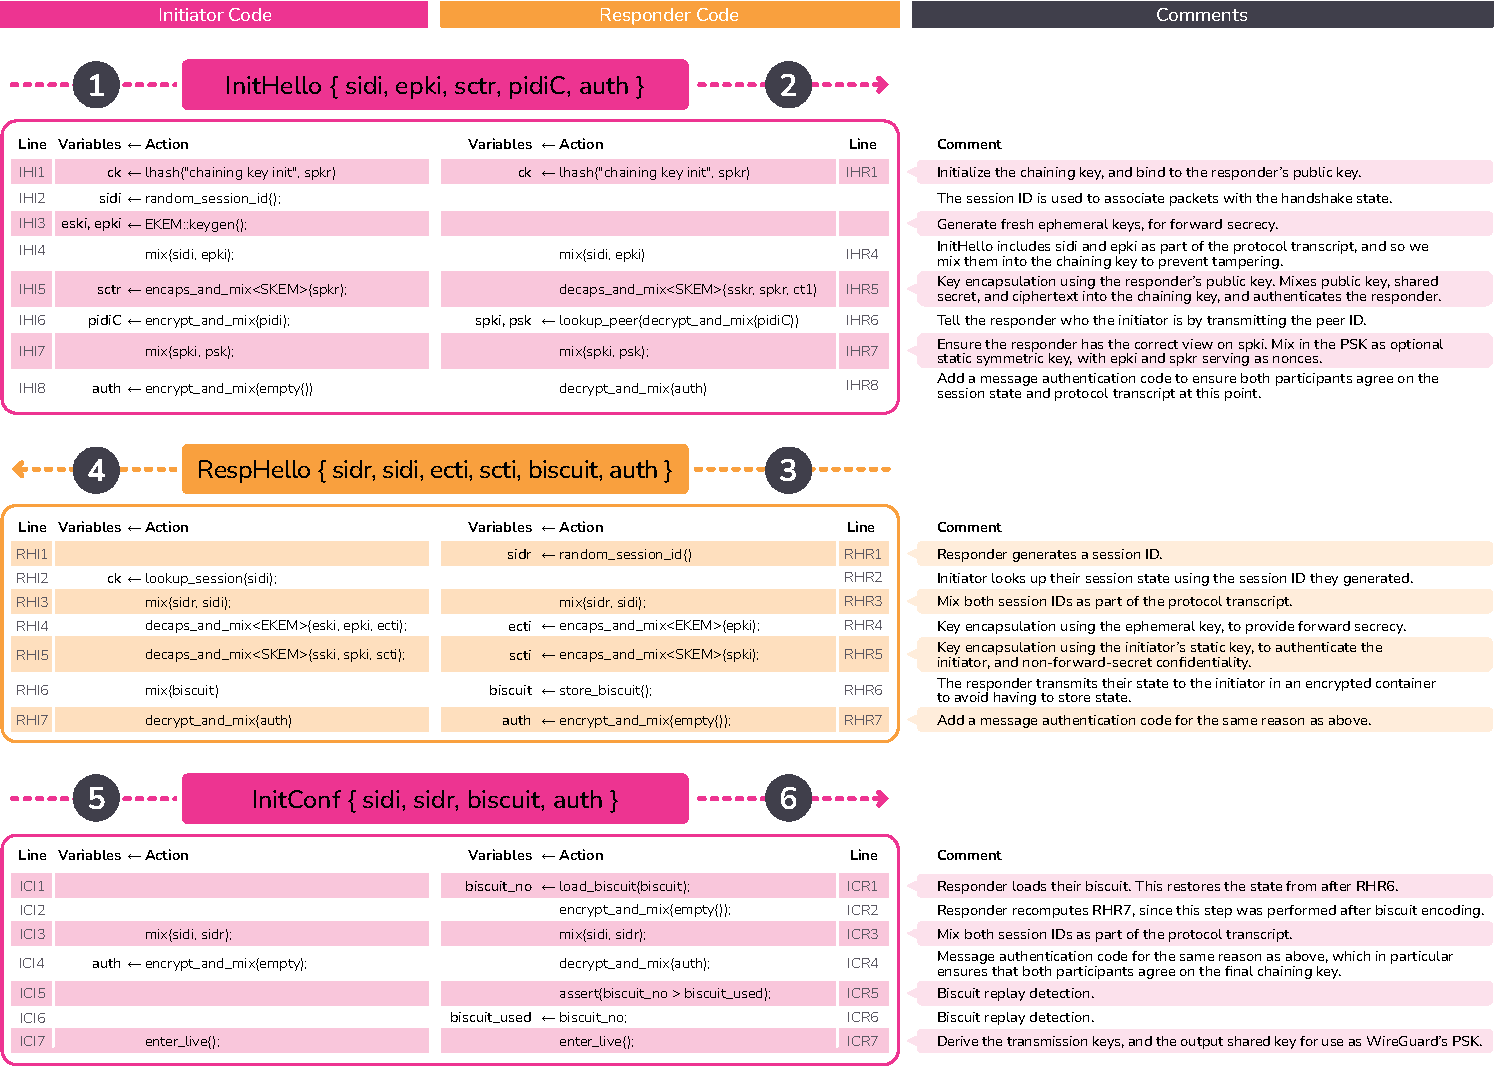
\includegraphics[height=.9\textheight]{graphics/rosenpass-wp-message-handling-code.pdf}
\end{frame}

\begin{frame}{Professional illustrators create stunning graphics}
  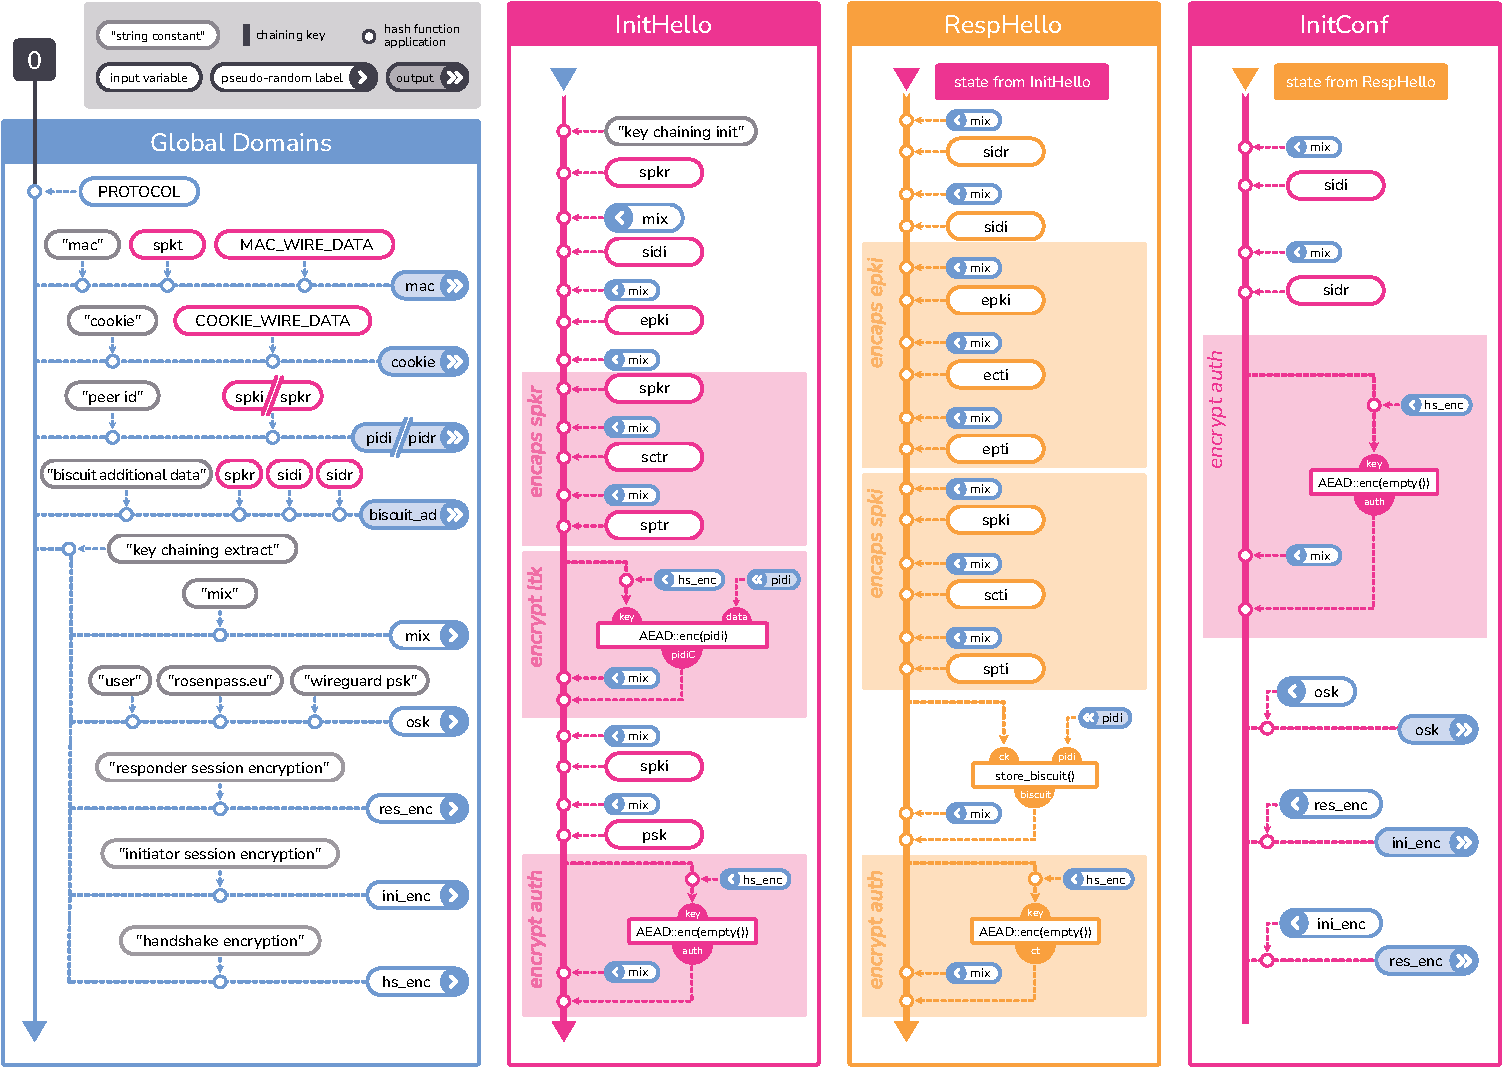
\includegraphics[height=.9\textheight]{graphics/rosenpass-wp-hashing-tree.pdf}
\end{frame}

\begin{frame}{Creating successful projects by knowing what not to do}
\begin{itemize}
  \item Rosenpass avoids targeting: GUIs, VPN data transport, support for many platforms
  \item Instead we: Created a core technology; working with companies to integrate Rosenpass (e.g. Open-Source VPN startups)
  \item \textbf{Vitally we} chose to focus on API; making it easy to integrate Rosenpass
  \item \textbf{Vitally we} integrate with the existing ecosystem (i.e. WireGuard) instead of trying to replace it
\end{itemize}
\end{frame}

\begin{frame}{Starting partnerships\dots}
\begin{itemize}
  \item with Open-Source VPN companies
  \item with Kubernetes VPN companies
  \item with Quantum-Key-Distribution Projects
  \item to verify the Rosenpass source code
  \item to apply isolation features to Rosenpass (Micro-VMs)
  \item with university teaching departments to use the project as a simple example of bleeding-edge modern crypto
\end{itemize}
\end{frame}

\begin{frame}{Talk to me about\dots}
\vspace{0.5cm}
\begin{itemize}
  \item using Rosenpass as demonstrator-project to integrate new cryptographic technologies in
  \item figuring out how to attract independent contributors to Formosa Projects
  \item applying API-focused techniques to Formosa projects to emphasize interoperability
  \item \textbf{Idea:} Providing XML-representations of proof assistants'\footnote{EasyCrypt, CryptoVerif, ProVerif, Tamarin} inputs and outputs to allow easy integration with external tools
  \item \textbf{Idea:} Python libraries to work with Formosa tools as everybody knows python
\end{itemize}
\vspace*{1.5cm}
\end{frame}

\end{document}

\printbibliography

\clearpage
\setcounter{framenumber}{\totalcontentframes}



\end{document}
